\documentclass[a4paper]{article}
\usepackage[ngerman]{babel}
\usepackage[T1]{fontenc}
\usepackage[utf8]{inputenc}
\usepackage{pdfpages}
\usepackage{a4wide}
\usepackage{amsmath}
\usepackage{amssymb}
\usepackage{graphics}
\usepackage{mathrsfs}
\usepackage{xspace}
\usepackage{verbatim}
\usepackage{float}
\usepackage{csvsimple}
\usepackage{pgfplotstable} % Generates table from .csv
\usepackage{setspace}
\restylefloat{table}
\providecommand{\zB}{z.\,B.\@\xspace}
\providecommand{\Matlab}{\textsc{Matlab}\xspace}
\usepackage[binary-units]{siunitx}
\sisetup{locale = DE}
\sisetup{per-mode = symbol-or-fraction}
\DeclareSIUnit\rounds{U}
\DeclareSIUnit\nmeter{Nm}
\usepackage[breaklinks=true]{hyperref}
\def \Stator {S}
\def \Rotor {R}
\renewcommand{\j}{\jmath}
% Ableitungen
\newcommand{\dd}{\mathop{}\!\mathrm{d}}
\newcommand{\Diff}[2]{\frac{\dd#1}{\dd#2}}
\newcommand{\DiffT}[1]{\Diff{#1}{t}}
\newcommand{\DDiff}[2]{\frac{\dd^2#1}{\dd#2^2}}
\newcommand{\DDiffT}[1]{\DDiff{#1}{t}}
\newcommand{\PartDiff}[2]{\frac{\partial #1}{\partial #2}}
\newcommand{\PartDiffT}[1]{\Diff{#1}{t}}
\newcommand{\PartDDiff}[2]{\frac{\partial^2 #1}{\partial #2^2}}
\newcommand{\PartDDiffT}[1]{\DDiff{#1}{t}}

% Makro für Gleichungen, Abbildungen, Tabellen
\newcommand{\abb}[1]{Abb. \ref{#1}}
\newcommand{\tab}[1]{Tab. \ref{#1}}
\newcommand{\glg}[1]{Glg. \ref{#1}}
\newcommand{\chp}[1]{Kap. \ref{#1}}
\usepackage[european]{circuitikz}
\usepackage{tikz}
\usetikzlibrary{arrows,decorations,intersections, decorations.text,calc}
\usepackage{pgfplots}
\pgfplotsset{compat=1.16}
\usepgfplotslibrary{units}
\pgfplotsset{ticklabel style={/pgf/number format/use comma,/pgf/number format/1000 sep={ }}}
\usetikzlibrary{external}
\tikzexternalize[prefix=tikz/,optimize command away=\includepdf]
%\tikzset{external/force remake}
\begin{document}
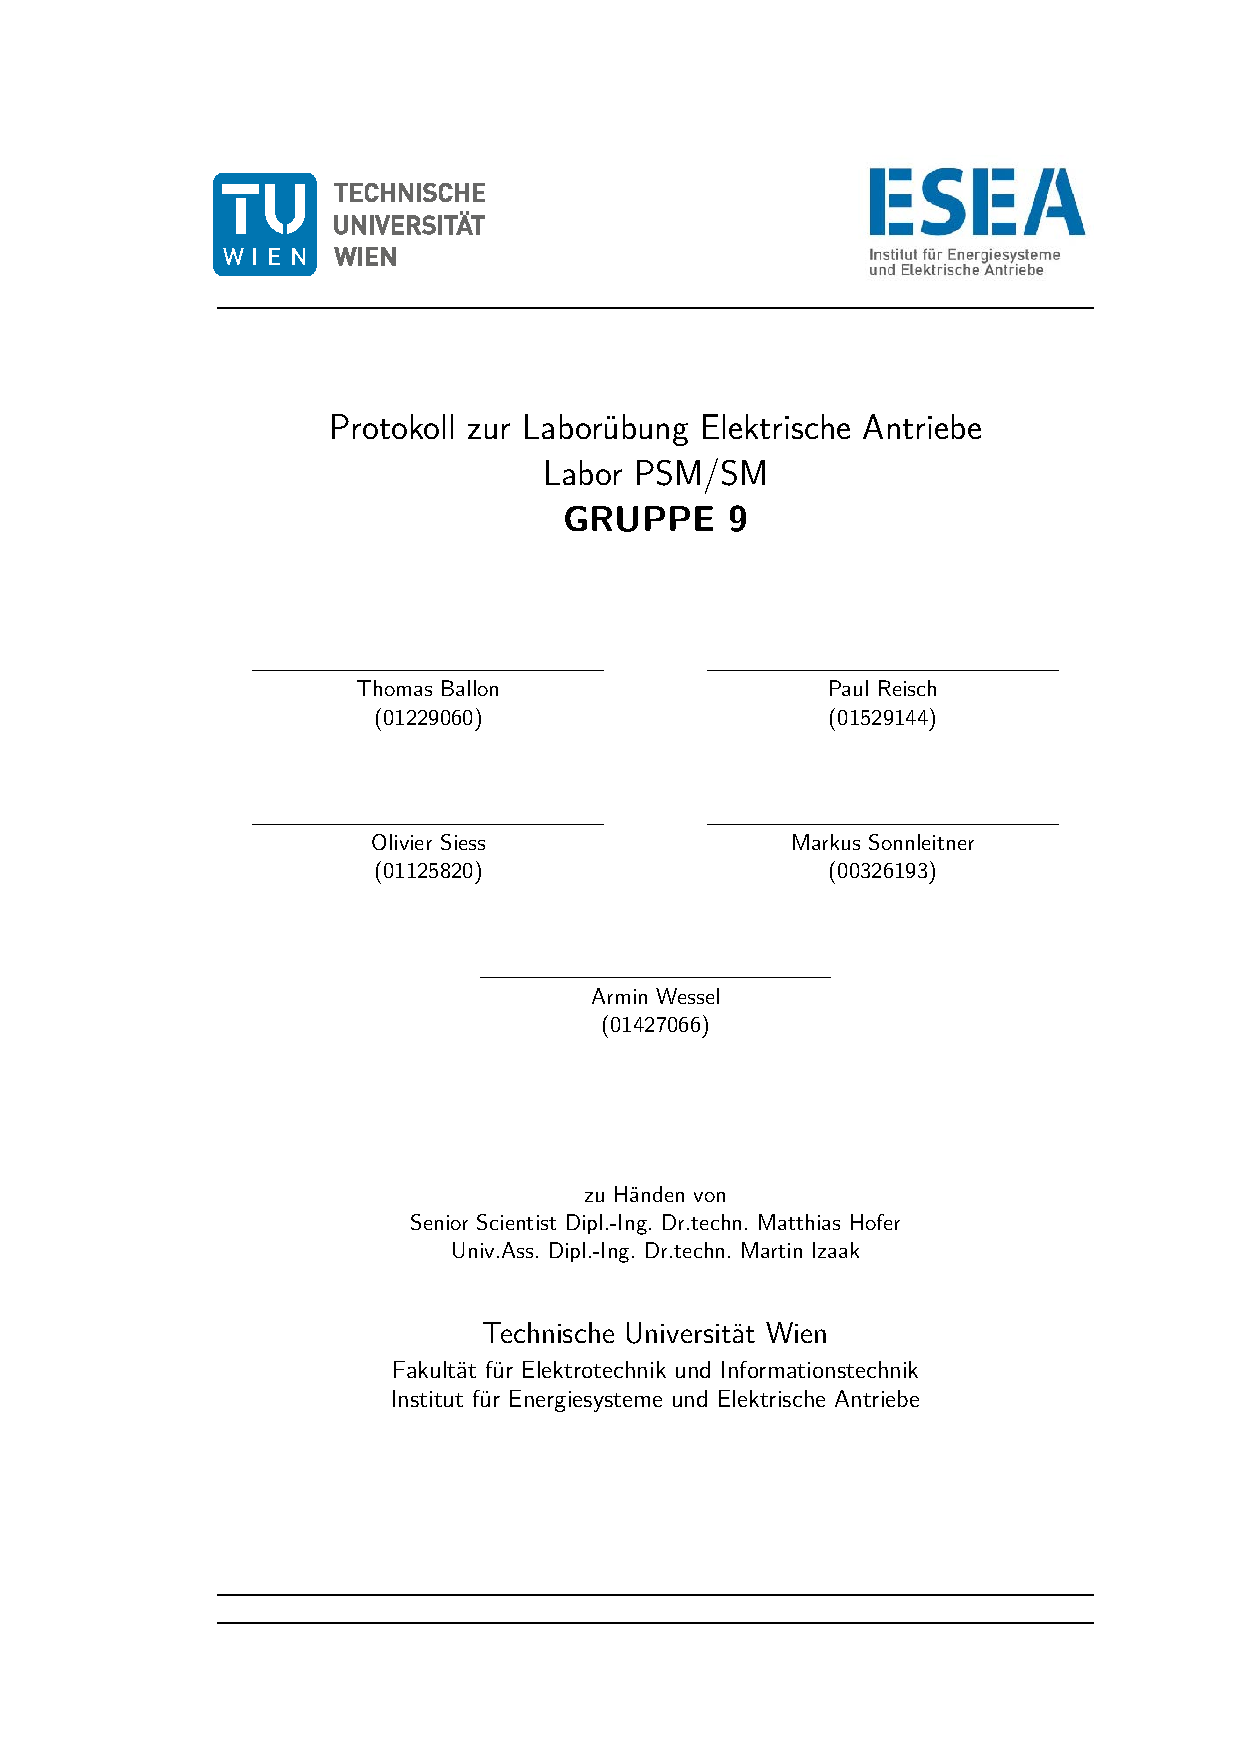
\includepdf{Deckblatt_PSM}
\tableofcontents\newpage
\section{PSM}
Lorem ipsum dolor sit amet, consectetur adipiscing elit. Mauris fringilla suscipit faucibus. Duis tincidunt, augue et dapibus lacinia, tortor mi viverra sapien, non ullamcorper odio risus a mauris. Maecenas at libero et mauris scelerisque sollicitudin quis sed orci. Donec congue ante felis, rutrum commodo lorem auctor quis. In consequat luctus turpis et vulputate. In sit amet rhoncus risus, porta imperdiet ex. Morbi neque lacus, consectetur quis dictum quis, pulvinar ac urna. Aliquam in dolor ut erat facilisis fringilla. Sed molestie commodo est.

Mauris sit amet eros sem. Donec quam massa, luctus ut nunc at, dignissim ornare augue. Aenean sagittis consequat nulla quis facilisis. Duis ultricies laoreet dui, ut condimentum arcu sodales sit amet. Nullam efficitur tellus vel faucibus scelerisque. Duis varius felis vitae eros maximus vestibulum. In porttitor pellentesque tellus, vel placerat orci. Phasellus consequat libero purus, sit amet semper ipsum fermentum non. Quisque rutrum sapien lectus, at faucibus eros egestas eget. Nulla id nisi tortor. Morbi porttitor interdum porta.

Morbi porta dolor metus, eget hendrerit justo ullamcorper ut. Vivamus commodo, arcu quis finibus eleifend, odio sem dignissim orci, nec pellentesque sapien metus at tortor. Sed dictum lectus suscipit imperdiet ultrices. Proin tellus neque, ornare sed mattis vel, faucibus at turpis. Lorem ipsum dolor sit amet, consectetur adipiscing elit. Morbi sit amet condimentum risus, nec lobortis sem. Donec molestie vel dui in egestas. Quisque tellus nisl, suscipit at viverra eget, aliquam eu est. Nam cursus nunc ultrices, pulvinar lorem vel, ullamcorper ante. Nunc sed dolor nec tellus commodo vehicula.

Phasellus id arcu sed enim sodales fringilla at nec metus. Mauris vel nibh et nibh bibendum gravida ut at metus. Sed bibendum, dui nec congue sodales, quam urna gravida lorem, sed vestibulum velit mi nec lorem. Quisque placerat congue ullamcorper. Vestibulum sollicitudin enim at risus gravida suscipit. Maecenas blandit consectetur enim, sed maximus diam dignissim at. Nam venenatis erat eleifend velit posuere accumsan. Nunc bibendum felis ac elit posuere venenatis. Suspendisse aliquet quam magna. Aenean quis ante posuere, interdum quam ut, accumsan ex.

Fusce molestie lacinia maximus. Suspendisse eget ex nec orci ullamcorper euismod auctor sed dui. Vivamus iaculis egestas tellus non consectetur. Sed dapibus vitae felis in gravida. Donec sapien sem, euismod et tincidunt egestas, bibendum eget odio. Nulla sed sapien efficitur, mattis metus ac, aliquam leo. Integer consequat bibendum turpis, at rhoncus purus sodales eget. Aenean quis accumsan velit.
\section{Anhang}
Lorem ipsum dolor sit amet, consectetur adipiscing elit. Mauris fringilla suscipit faucibus. Duis tincidunt, augue et dapibus lacinia, tortor mi viverra sapien, non ullamcorper odio risus a mauris. Maecenas at libero et mauris scelerisque sollicitudin quis sed orci. Donec congue ante felis, rutrum commodo lorem auctor quis. In consequat luctus turpis et vulputate. In sit amet rhoncus risus, porta imperdiet ex. Morbi neque lacus, consectetur quis dictum quis, pulvinar ac urna. Aliquam in dolor ut erat facilisis fringilla. Sed molestie commodo est.

Mauris sit amet eros sem. Donec quam massa, luctus ut nunc at, dignissim ornare augue. Aenean sagittis consequat nulla quis facilisis. Duis ultricies laoreet dui, ut condimentum arcu sodales sit amet. Nullam efficitur tellus vel faucibus scelerisque. Duis varius felis vitae eros maximus vestibulum. In porttitor pellentesque tellus, vel placerat orci. Phasellus consequat libero purus, sit amet semper ipsum fermentum non. Quisque rutrum sapien lectus, at faucibus eros egestas eget. Nulla id nisi tortor. Morbi porttitor interdum porta.

Morbi porta dolor metus, eget hendrerit justo ullamcorper ut. Vivamus commodo, arcu quis finibus eleifend, odio sem dignissim orci, nec pellentesque sapien metus at tortor. Sed dictum lectus suscipit imperdiet ultrices. Proin tellus neque, ornare sed mattis vel, faucibus at turpis. Lorem ipsum dolor sit amet, consectetur adipiscing elit. Morbi sit amet condimentum risus, nec lobortis sem. Donec molestie vel dui in egestas. Quisque tellus nisl, suscipit at viverra eget, aliquam eu est. Nam cursus nunc ultrices, pulvinar lorem vel, ullamcorper ante. Nunc sed dolor nec tellus commodo vehicula.

Phasellus id arcu sed enim sodales fringilla at nec metus. Mauris vel nibh et nibh bibendum gravida ut at metus. Sed bibendum, dui nec congue sodales, quam urna gravida lorem, sed vestibulum velit mi nec lorem. Quisque placerat congue ullamcorper. Vestibulum sollicitudin enim at risus gravida suscipit. Maecenas blandit consectetur enim, sed maximus diam dignissim at. Nam venenatis erat eleifend velit posuere accumsan. Nunc bibendum felis ac elit posuere venenatis. Suspendisse aliquet quam magna. Aenean quis ante posuere, interdum quam ut, accumsan ex.

Fusce molestie lacinia maximus. Suspendisse eget ex nec orci ullamcorper euismod auctor sed dui. Vivamus iaculis egestas tellus non consectetur. Sed dapibus vitae felis in gravida. Donec sapien sem, euismod et tincidunt egestas, bibendum eget odio. Nulla sed sapien efficitur, mattis metus ac, aliquam leo. Integer consequat bibendum turpis, at rhoncus purus sodales eget. Aenean quis accumsan velit.
\end{document}